\documentclass[12pt,a4paper]{article}
\usepackage[colorlinks=true, urlcolor=blue, linkcolor=red]{hyperref}
\usepackage{amsmath, amssymb, amsthm, algorithm, booktabs, listings}
\usepackage[dvipsnames,usenames]{xcolor}
\usepackage[noend]{algpseudocode}
\usepackage{tikz}
\usepackage{fancyhdr}
\usepackage{geometry}
\newgeometry{top=2cm, bottom=2cm, left=1.5cm, right=1.5cm}
\usepackage[shortlabels]{enumitem}
\usepackage{cleveref}
\usepackage{mdframed}
\usepackage[most]{tcolorbox}
\hypersetup{citecolor=blue}
\usepackage{times}
\usepackage{subcaption}
\theoremstyle{definition}
\newtheorem{definition}{Definition}[subsection]
\newtheorem{statement}{Statement}[subsection]
\usepackage[backend=biber,style=alphabetic,sorting=ynt]{biblatex}
\hypersetup{linkcolor=black}
\addbibresource{references.bib}
\pagestyle{fancy}
\defbibheading{blueboxed}{%
  \begin{tcolorbox}[colframe=blue!50!black, colback=blue!20]
    \section{References}
  \end{tcolorbox}
}

\newcommand{\bluebox}[1]{%
  \begin{tcolorbox}[colframe=blue!50!black, colback=blue!20]
    #1
  \end{tcolorbox}%
}

\newcommand{\purplebox}[1]{%
  \begin{tcolorbox}[colframe=violet!80!black, colback=violet!20]
    #1
  \end{tcolorbox}%
}

\newcommand{\pinkbox}[2]{%
  \begin{tcolorbox}[colframe=magenta!50!black, colback=magenta!20, title={#1}]
    #2
  \end{tcolorbox}%
}

\newcommand{\bluebigbox}[2]{%
  \begin{tcolorbox}[colframe=blue!50!black, colback=blue!20, title={#1}, toptitle=5pt, bottomtitle=5pt]
    #2
  \end{tcolorbox}%
}

\newcommand{\bluesec}[1]{%
  \bluebox{\section*{#1}}
}

\newcommand{\purplesec}[1]{%
  \purplebox{\subsection*{#1}}
}

\DeclareRobustCommand{\hlit}[1]{\colorbox{yellow}{\textit{#1}}}
\DeclareRobustCommand{\hlbf}[1]{\colorbox{yellow}{\textbf{#1}}}
\DeclareRobustCommand{\hl}[1]{\colorbox{yellow}{#1}}
\DeclareRobustCommand{\ghl}[1]{\colorbox{green}{#1}}
\DeclareRobustCommand{\lghl}[1]{\colorbox{green!20}{#1}}
\newcommand{\bs}{\textbackslash}
\newcommand{\boxtxt}[1]{\boxed{\text{#1}}}

\tcbuselibrary{listings}
\newtcblisting{shuncode}{
    listing only,
    listing options={
        language=C,
        basicstyle=\ttfamily\small,
        keywordstyle=\color{blue},
        commentstyle=\color{green!50!black},
        stringstyle=\color{red}
    },
    colback=cyan!10,
    colframe=cyan!80!black,
    boxrule=2pt,
    left=0pt,
    right=0pt,
    top=0pt,
    bottom=0pt,
    boxsep=0pt,
    arc=5pt,
    enhanced
}

\newtcblisting{shuncmd}[1][]{
  listing only,
  listing options={
    language=bash,
    basicstyle=\ttfamily\small,
    keywordstyle=\color{blue},
    commentstyle=\color{green!50!black},
    stringstyle=\color{red},
    breaklines=true
  },
  colframe=cyan!80!black,
  colback=cyan!10,
  title={#1},
  enhanced,
}

\lhead{Complex Analysis}
\chead{Midterm Theorems}
\rhead{Shun (@shun4midx)}

\begin{document}
\begin{center}
  {\Large \bf Complex Analysis: Midterm Theorems}\\[8pt]
  \textbf{Author:} Shun (@shun4midx)
\end{center}

\pinkbox{Remark}{
  I only will include theorems that are useful for me, i.e. things that I still find useful, or whose proofs I'm shaky on, after learning this course for 7 weeks. Otherwise, there will be too many theorems. For me, my dyslexic brain is only able to memorize something if I rewrite it because I can't really read, why I have to retype this many proofs.
}

\vspace{1.0em}\bluesec{Power Series}

\purplesec{Analytic Polynomial}

\pinkbox{Proposition}{
  A polynomial $P(x, y)$ is \hl{\textbf{analytic} $\Leftrightarrow P_y = iP_x$}
}

\begin{proof}
  ``$\Rightarrow$'': By def, $\exists\ \alpha_k \in \mathbb{C},\ N \in \mathbb{N}$, s.t. \lghl{$P(x, y) = \sum_{k = 0}^N \alpha_k (x + iy)^k$}. Then, $P_y = \sum_{k = 1}^N k \alpha_k (x + iy)^{k - 1} i$, $P_x = \sum_{k = 1}^N k \alpha_k (x + iy)^{k - 1}$, so $P_y = iP_x$. \\

  \noindent ``$\Leftarrow$'': We can rewrite $P(x, y) = \sum_{k = 0}^N Q^k(x, y)$, where we have polynomials in the form \\ \lghl{$Q^k(x, y) = c_0 x^k + c_1 x^{k - 1}y + \dots + c_k y^k$}. \\

  \noindent From assumption, $Q_y^k = iQ_x^k\ \forall\ k$. Hence, \lghl{$\sum_{p = 1}^k p c_p x^{k - p} y^{p - 1} = \sum_{p = 0}^{k - 1} (k - p)c_p x^{k - p - 1} y^p i$}

  \begin{itemize}
    \item $p = 1$: $1c_1 = ik c_0 \Rightarrow c_1 = {k \choose 0} c_0$
    \item $p = 2$: $2c_2 = (k - 1) c_1 i \Rightarrow c_2 = i^2 \frac{k(k - 1)}{2} c_0$
    \item For any $p > 1$, $pc_p = (k - p + 1) c_{p - 1} i \Rightarrow$ \lghl{$c_p = i^p {k \choose p} c_0$}
  \end{itemize}

  \noindent Hence, \lghl{$Q^k = \sum_{p = 0}^k i^p {k \choose p} c_0 x^{k - p} y^p = c_0(x + iy)^k\ \forall k$}, so $P$ is \textbf{analytic}.
\end{proof}

\vspace{1.0em}\purplesec{Radius of Convergence}

\pinkbox{Theorem}{
  Given the power series $\sum_{k = 0}^\infty c_k z^k = f(z)$, define \hl{$L := \limsup_{k \to \infty} |c_k|^{\frac{1}{k}}$}, then we have:

  \begin{enumerate}
    \item $L = 0 \Rightarrow P(z)$ converges $\forall z \in \mathbb{C}$
    \item \hl{$L = \infty$} $\Rightarrow P(z)$ converges only at \hl{$z = 0$}
    \item \hl{$0 < L < \infty$} $\Rightarrow P(z)$ converges on \hl{$|z| < \frac{1}{L}$} and diverges on $|z| > \frac{1}{L}$
  \end{enumerate}
}

\begin{proof}
  We consider the three cases separately.
  \begin{enumerate}
    \item Hence, given any $z \in \mathbb{C}$, $\limsup_{k \to \infty} |c_k|^\frac{1}{k} = 0$. By def, take \lghl{$\varepsilon = \frac{1}{2}$}, $\exists\ N$, s.t. $k > N \Rightarrow$ \lghl{$|c_k|^\frac{1}{k} |z| < \frac{1}{2}$} $\Rightarrow \sum |c_k z^k| =$ \lghl{$\sum(|c_k|^\frac{1}{k}|z|)^k < \sum (\frac{1}{2})^k = 1$}
    \item Consider small $|z|$, $\forall\ N \in \mathbb{N},\ \exists\ k > N$, s.t. \lghl{$|c_k|^\frac{1}{k} > \frac{1}{|z|} \Rightarrow |c_k z^k| > 1$}, so $P(z)$ only converges when $z = 0$
    \item Take $R = \frac{1}{L}$, \lghl{$|z| = R(1 - \delta)$}, i.e. $1 > \delta > 0$ when $|z| < \frac{1}{L}$. Then, $\forall\ \varepsilon > 0, \exists N \in \mathbb{N},\ n > N$, s.t. \lghl{$|z|(L - \varepsilon) \leq |z|\sup_{k \geq n} |c_k|^\frac{1}{k} \leq |z|(\varepsilon + L)$} $ < 1 + \varepsilon R (1 - \delta) - \delta < 1 - \frac{\delta}{2}$, so it is \textbf{abs conv} \\
    
    \noindent If $|z| > R$, $\limsup |c_k|^\frac{1}{k}|z| > 1 \Rightarrow$ \lghl{for inf values of $k$, $|c_k z^k| > 1 \Rightarrow \sum c_k z^k$ div}
  \end{enumerate}
\end{proof}

\purplesec{Differentiation}

\pinkbox{Theorem}{
  Given a power series $P(z) = \sum_{k = 0}^\infty c_k z^k$ with radius of convergence $R$, then $P'(z)$ exists on \hl{$|z| < R$, $P'(z) = \sum_{k = 1}^\infty k c_k z^{k - 1}$}
}

\begin{proof}
  For $0 < R < \infty$, let $|z| = R - \delta$, $R \geq \delta > 0$. WLOG, consider \lghl{$|h| < \frac{\delta}{2}$} and consider \lghl{$\frac{P(z + h) - P(z)}{h}$}. \\

  \vspace{1.0em}\noindent $\frac{P(z + h) - P(z)}{h} = \frac{1}{h} \sum c_k((z + h)^k - z^k) =$ \lghl{$\sum_{k = 1}^\infty k c_k z^{k - 1} + \sum_{k = 2}^\infty c_k b_k$}, where $b_k = \sum_{p = 2}^k {k \choose p} h^{p - 1} z^{k - p}$ \\

  \begin{itemize}
    \item If \lghl{$|z| = 0$, $b_k = h^{k - 1}$} $\Rightarrow$ \lghl{$\sum c_k h^{k - 1} < \infty \Rightarrow \sum c_k h^{k - 1} \to 0$ as $h \to 0$}
    \item If $|z| \neq 0$, \lghl{${k \choose p} \leq {k \choose {p - 2}} k^2$}. \\
    
    Hence, \lghl{$|b_k| \leq \frac{|h|}{|z|^2} k^2 \sum_{p = 2}^k {k \choose p - 2} |h|^{p - 2} |z|^{k - (p - 2)} \leq \frac{|h|}{|z|^2} k^2 \sum_{j = 0}^k {k \choose j} |h|^j |z|^{k - j}$} $= \frac{|h|}{|z|^2} k^2 (|z| + |h|)^k \leq \frac{|h|}{|z|^2} k^2 (R - \frac{\delta}{2})^k$ \\

    Thus, $|\sum_{k = 2}^\infty c_k b_k| \leq \frac{|h|}{|z|^2} k^2 |c_k| (R - \frac{\delta}{2})^k \to 0$
  \end{itemize}

  \noindent The remaining case is simple for $R = \infty$, we apply the case above and show it holds for any $R$.
\end{proof}

\pinkbox{Corollary}{
  Power series are \textbf{smooth in their domain of convergence}
}

\purplesec{Uniqueness}

\pinkbox{Theorem}{
  If $\exists \{z_n\}_n \to 0$, and $\sum c_k z_n^k = 0$, then $c_k = 0\ \forall k$
}

\begin{proof}
  As $P$ is \textbf{conti}, thus \lghl{$P(0) = \lim_{n \to \infty} P(z_n) = 0 \Rightarrow c_0 = 0$.} \\

  \noindent Consider, \lghl{$g(z) = \frac{f(z)}{z}$} with the \textbf{same radius of convergence} as $f(z)$. Similarly, $g(0) = \lim_{n \to \infty} \frac{f(z_n)}{z_n} = 0 \Rightarrow c_1 = 0$. {\textcolor{red}{Note that this can be recusrively applied.}} \\

  \noindent $\therefore$ By induction on $n$, $c_n = 0\ \forall n$.
\end{proof}

\pinkbox{Corollary}{
  If \hl{$\sum a_k z^k$ and $\sum b_k z^k$ agree} on $\{z_n\}_n$ as $n \to \infty$, then \hl{$a_k = b_k\ \forall k$}
}

\vspace{1.0em}\bluesec{Analytic Functions}

\pinkbox{Proposition}{
  If $f = u + iv$ is differentiable at $z$, then $f_x$ and $f_y$ exist and satisfy the CR-equation $f_y = if_x$
}

\begin{proof}
  By def, $f$ is diff $\Rightarrow \lim_{h \to 0}\frac{f(z + h) - f(z)}{h}$ exists. Along the \textbf{real} axis, this limit is \lghl{$\lim_{\xi \to 0} \frac{f(x + \xi, y) - f(x, y)}{\xi}$} \lghl{$= f_x$}. Along the \textbf{imaginary} axis, this limit is \lghl{$\lim_{\xi \to 0} \frac{f(x, y + \xi) - f(x, y)}{\xi i} = \frac{f_y}{i}$}. Hence, $f_x = \frac{f_y}{i} \Rightarrow \boxed{f_y = if_x}$
\end{proof}

\pinkbox{Counterexample for $f_x$ and $f_y$ exist at $z$ and $f_y = if_x$, but $f$ is not differentiable}{
  \[
  f(z) =
  \begin{cases}
    \colorbox{yellow}{$\dfrac{xy(x + iy)}{x^2 + y^2}$}, & z \neq 0 \quad {\textcolor{red}{(\text{i.e. } xy \cdot \tfrac{z}{|z|})}} \\[6pt]
    0, & z = 0 \quad (\Leftrightarrow (x, y) = 0)
  \end{cases}
  \]

  We notice, both on the \textbf{x-axis and y-axis}, we have $f(z) \equiv 0$, hence \hl{$f_x(0) = f_y(0) = 0$}. \\

  However, along \hl{$y = ax$} for $a \neq 0$, we get $f(x, ax) = \frac{a(1 + ia)}{1 + a^2}x \Rightarrow$ \hl{$\lim_{x \to 0} \frac{f(x, ax) - f(0, 0)}{x + axi} = \frac{a}{1 + a^2} \neq 0$}. \\

  Hence, $\lim_{h \to 0} \frac{f(z + h) - f(z)}{h}$ does not exist, so $f$ is NOT differentiable. \qed
}

\pinkbox{Proposition}{
  Suppose that $f_x$ and $f_y$ exist in a \textbf{nbd of} $\mathbf{z}$ and are \textbf{conti} at $z$. If $f$ satisfies the CR-eq, then $f$ is \textbf{differentiable}.
}

\begin{proof}
  Say $z = x + iy,\ h = \xi + i \eta$, and $f(z) = u(z) + iv(z)$. \\

  \noindent Then, $\frac{f(z + h) - f(z)}{h} = \frac{[u(x + \xi, y + \eta) - u(x, y)]}{\xi + i \eta} + i \frac{[v(x + \xi, y + \eta) - v(x, y)]}{\xi + i \eta}$ \\

  \noindent By MVT with ``$-u(x + \xi, y) + u(x + \xi, y)$'' and $-v(x + \xi, y) + v(x + \xi, y)$, this equals:

  \noindent \lghl{$\frac{\eta}{\xi + i\eta} [\frac{u(x + \xi, y + \eta) - u(x + \xi, y)}{\eta} + i\frac{v(x + \xi, y + \eta) - v(x + \xi, y)}{\eta}] + \frac{\xi}{\xi + i\eta}[\frac{u(x + \xi, y) - u(x, y)}{\xi} + i\frac{v(x + \xi, y) - v(x, y)}{\eta}]$} \\

  $= \frac{\eta}{\xi + i\eta}[u_y(x + \xi, y + \theta_1 \eta) + iv_y(x + \xi, y + \theta_2 \eta)] + \frac{\xi}{\xi + i\eta}[u_x(x + \theta_3\xi, y) + iv_x(x + \theta_4\xi, y)]$ \\

  \noindent As we know, $0 < \theta_k < 1$, and $|\frac{\eta}{\xi + i\eta}| = |\frac{\Re(h)}{h}| \leq 1$, $|\frac{\xi}{\xi + i \eta}| \leq 1$. \\

  \noindent \textbf{Claim:} $\lim_{h \to 0} \frac{f(z + h) - f(z)}{h} = f_x(z)$ \\

  \begin{proof}
    We know, by CR-eq, \lghl{$f_x(z) = \frac{\xi}{\xi + i\eta} f_x(z) + \frac{\eta}{\xi + i\eta} f_y(z)$} \\

    \noindent As $f_x$ and $f_y$ are conti, \lghl{$\frac{f(z + h) - f(z)}{h} - f_x(z) = \frac{\eta}{\xi + i\eta}[(u_y(x + \xi, y + \theta_1 \eta) - u_y(x, y)) + i(v_y(x + \xi, y + \theta_2 \eta)$} \lghl{$- v_y(x, y))] + \frac{\xi}{\xi + i\eta}[(u_x(x + \theta_3\xi, y) - u_x(x, y)) + i(v_x(x + \theta_4\xi, y) - v_x(x, y))] \to 0$} as $h$, i.e. $\xi,\ \eta \to 0$.
  \end{proof}

  \noindent Hence, $f$ is \textbf{diffable} and $\boxed{f'(z) = f_x(z)}$
\end{proof}

\vspace{1.0em}\bluesec{Applications of CR Equation}

\purplesec{Regions}

\pinkbox{Region Implies Connecting Vertical and Horizontal Line Segments}{
  If $D$ is a \textbf{region}, then $\forall x, y \in D, \exists$ a curve consisting of horizontal and vertical \hl{line segments that} \hl{connect $x$ and $y$}
}

\begin{proof}
  For any $x \in D$, say $U_x := \{y \in D\ |\ x \text{ connects to } y \text{ via vertical/horizontal line segments that connect}\}$

  \begin{enumerate}
    \item \lghl{``$U_x$ is open''}: For all $y \in U_x \subseteq D$, as $D$ is open, $\exists$ \lghl{open disk $B_\delta(y) \subseteq D$}. As $\forall a \in B_\delta(y)$, $a$ can be connected to $y$ by vertical/horizontal line segments, thus $x \to y \to a$ can be connected via these line segments, so \lghl{$B_\delta(y) \subseteq U_x$}.
    \item \lghl{``$D \setminus U_x$ is open''}: For $y \in D \setminus U_x$, $D$ is open $\Rightarrow \exists$ open disk $B_\delta(y) \subseteq D \Rightarrow$ \lghl{$B_\delta(y) \cap U_x = \emptyset \Rightarrow$} \lghl{$B_\delta(y) \subseteq D \setminus U_x$}
  \end{enumerate}

  \noindent Combining (1), (2), and that $D$ is connected, hence we get $\boxed{D = U_x}$.
\end{proof}

\pinkbox{$u$ is constant implies $f$ is constant}{
  If $f = u + iv$ is \textbf{analytic} on a region $D$ and $u$ is constant, then $f$ is constant
}

\begin{proof}
  $u$ is constant $\Rightarrow u_x = u_y = 0$. \lghl{By \textbf{CR-eq}, $v_x = v_y = 0$}. \\

  \noindent As $D$ is a region, thus $\forall a, b \in D$, \lghl{$\exists$ a horizontal/vertical connected path connecting $a$ and $b$}. Hence, $f(a) = f(b)$ (for all $a, b \in D$), so f is \textbf{constant}.
\end{proof}

\vspace{1.0em}\bluesec{Line Integrals}

\pinkbox{Smoothly Equivalent Integrals are Equivalent}{
  If $\boxed{C_1 \sim_{sim} C_2}$, then \hl{$\int_{C_1} f(z) dz = \int_{C_2} f(z) dz$}.
}

\begin{proof}
  We set $f(z) = u(z) + iv(z)$ and $z = x(t) + iy(t)$. \\

  \noindent Then, we know $\int_{C_1} f(z) dz = \int_a^b f(z(t)) z'(t) dt$ 
  
  \lghl{$= \int_a^b[u(z(t))x'(t) - v(z(t))y'(t)] dt + i \int_a^b[u(z(t))y'(t) + v(z(t))x'(t)] dt$} \\

  \noindent With \lghl{$\int_c^d u(z(\lambda(t))) x'(\lambda(t)) \lambda'(t) dt = \int_a^b u(z(t)) x'(t) dt$}, substitute it back in and going in the opposite direction, we prove the equation.
\end{proof}

\vspace{0.5em}\pinkbox{Lemma on Modulus of Integral}{
  Let $t \in \mathbb{R}$, $G(t)$ be a continuous complex-valued function. Then, \hl{$|\int_a^b G(t) dt| \leq \int_a^b |G(t)| dt$}
}

\begin{proof}
  Set \lghl{$R(t) e^{i \theta} := \int_a^b G(t) dt$}, for some fixed $\theta \in \mathbb{R}$, $R \in \mathbb{R}_{\geq 0}$. \\

  \noindent Then, $R = |\int_a^b G(t) dt| = \int_a^b e^{-i\theta} G(t)dt = \int_a^b A(t) dt + i \int_a^b B(t) dt$. By \textbf{comparing like terms}, we deduce \lghl{$R = \int_a^b A(t) dt$}. Hence, $R = \int_a^b A(t) dt \leq \int_a^b |A(t)| dt \leq \int_a^b |e^{-i\theta} G(t)| dt = \int_a^b |G(t)| dt$
\end{proof}

\pinkbox{ML-Formula}{
  Let $C$ be a \textbf{smooth} curve of \hl{length $L$}, and $f$ be conti on $C$ and \hl{$f << M$} throughout $C$. Then, \hl{$\int_C f(z) dz << ML$}
}

\begin{proof}
  Let $C$ be $z(t) = x(t) + iy(t)$ for some $t \in [a, b]$. Then, $\int_C f(z) dz = \int_a^b f(z(t)) z'(t) dt$. \\ 
  
  \noindent By the previous lemma, $\int_C f(z) dz <<$ \lghl{$\int_a^b |f(z(t))||z'(t)| dt \leq M \int_a^b |z'(t)| dt = ML$} (integrating $|z'(t)|$ was the formula for arc-length)
\end{proof}

\pinkbox{ML is the Tight Bound}{
  For $f(z) = \frac{1}{z}$, $C: \cos \theta + i \sin \theta$, then $\int_C f(z) dz = 2\pi i \Rightarrow |\int_C f(z) dz| = 2\pi = ML$
}

\pinkbox{Proposition (Limits)}{
  Suppose $\{f_n\}$ is a sequence of continuous functions and \hl{$f_n \to f$ unif} on a smooth curve $C$. Then, \hl{$\lim_{n \to \infty} \int_C f_n(z) = \int_C f(z) dz$}
}

\begin{proof}
  By def, $f_n \to f$ unif on $C$ means ``Given $\varepsilon > 0$, $\exists N$, s.t. $\forall n \geq N,\ |f_n(z) - f(z)| < \varepsilon\ \forall z \in C$'' \\

  \noindent Hence, $|\int_C f_n(z) dz - \int_C f(z) dz| = |\int_C (f_n - f)(z) dz| < \varepsilon\ \cdot\ \text{len}(C)\ \forall n \geq N$. (By ML-formula)
\end{proof}

\pinkbox{FTC Variant}{
  Let $F$ be an analytic function, $f = F'(z)$ and a smooth curve $C: z(t) = x(t) + iy(t)$, $t \in [a, b]$. Then, \hl{$\int_C f(z)dz = F(z(b)) - F(z(a))$}
}

\begin{proof}
  Let \lghl{$\gamma(t) := F(z(t)) = A(t) + iB(t)$}. As $F$ is analytic, by the chain rule, \lghl{$\gamma'(t) = F'(z(t)) z'(t)$}. \\

  \noindent Then, $\int_C f(z) dz = \int_a^b F'(z(t))z'(t) dt = \int_a^b \gamma'(t)dt = \boxed{\gamma(b) - \gamma(a)}$
\end{proof}

\purplesec{Rectangle Theorem}

\pinkbox{Lemma}{
  If $f$ is a \textbf{linear function}, i.e. $f = a + zb$, for $a, b \in \mathbb{C}$, and $\Gamma$ is the \textbf{boundary of a rectangle}, then \hl{$\int_\Gamma f(z) dz = 0$}
}

\begin{proof}
  \vspace{-1.0em}\begin{figure}[h]
    \centering
    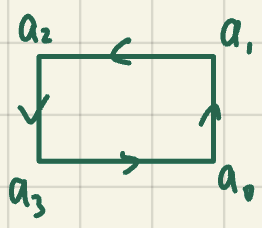
\includegraphics[width=0.12\textwidth]{img/rect.png}
  \end{figure}
  Say $\Gamma: z(t), a = a_0 \leq t \leq b = a_3$, and \lghl{$f = F'(z) \Rightarrow F := \frac{a}{2}z^2 + bz$} (since $f$ is ana on $\mathbb{C}$). Hence, we deduce $\int_\Gamma f(z) dz = \int_\Gamma F'(z)dz = $ \lghl{$F(z(b)) - F(z(a)) = 0$} (because $z(b) = z(a)$).
\end{proof}

\pinkbox{Rectangle Theorem}{
  Let $f$ be an \textbf{entire function}, and $\Gamma$ as above. Then, \hl{$\int_\Gamma f(z) dz = 0$}
}

\begin{proof}
  Let $I = \int_\Gamma f(z) dz$. Assume $f \neq 0$, otherwise $f = 0 \Rightarrow I = 0$. In this case, we divide $R$ as follows:

  \begin{figure}[h]
    \centering
    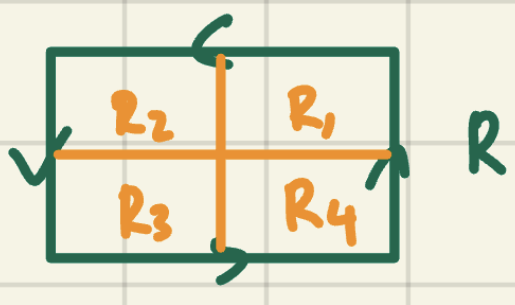
\includegraphics[width=0.15\textwidth]{img/divided_rect.png}
  \end{figure}

  \noindent Then, $\exists R_i$, s.t. \lghl{$|\int_{\Gamma_i} f(z) dz| \geq \frac{|I|}{4}$}, where $\Gamma_i$ is the boundary of $R_i$. Define \lghl{$R^{(1)}$ to be said $R_i$}. Continuing this process, we get $R^{(1)} \supseteq R^{(2)} \supseteq \dots$. Let \lghl{$z_0 \in \cap_{i = 1}^\infty R^{(i)}$}. \\

  \noindent As $f$ is entire, thus $f$ is \textbf{analytic} at $z_0$. By def, $\forall\ \varepsilon > 0,\ \exists\ \delta > 0$, s.t. $|h| < \delta \Rightarrow$ \lghl{$|\frac{f(z_0 + h) - f(z_0)}{h} - f'(z_0)| < \varepsilon$}. Hence, for some $|\varepsilon(z)| \leq \varepsilon$, we can have \lghl{$f(z) = f(z_0) + f'(z_0)(z - z_0) + \varepsilon(z)(z - z_0)$}. \\

  \noindent Note that $f(z_0) + f'(z_0)(z - z_0)$ is \textbf{linear}. Thus, we can choose $N$ s.t. $\forall n \geq N$, we have $|z - z_0| < \delta \Rightarrow$ \lghl{$\int_{\Gamma^{(n)}} f(z) dz = \int_{\Gamma^{(n)}} \epsilon(z)(z - z_0) dz$}. \\

  \noindent Let $s$ be the length of the longest side of $R$. We know \lghl{$|\Gamma^{(n)}| \leq \frac{4s}{2^n}$ and $|\varepsilon(z) (z - z_0)| < \varepsilon \cdot \frac{\sqrt{2} s}{2^n}$}. Thus, by ML formula, \lghl{$\int_{\Gamma^{(n)}} f(z) dz << \varepsilon \frac{4\sqrt{2} s^2}{4^n}$}. \\

  \noindent By our assumption, $|\int_{\Gamma^{(n)}} f(z) dz| \geq \frac{|I|}{4^n}$, hence \lghl{$|I| \leq \varepsilon \cdot 4\sqrt{2}s^2\ \forall \varepsilon > 0$}, hence $I = 0$.
\end{proof}

\pinkbox{Integral Theorem}{
  If $f$ is entire, then $f$ is everywhere the \textbf{derivative of an analytic function}. That is, $\exists$ an entire $F$ s.t. $F'(z) = f(z)\ \forall z$.
}

\begin{proof}
  Consider \lghl{$F(z) = \int_C f(\eta) d\eta$}, where $C: 0 \to \Re(z) \to z$.

  \begin{figure}[h]
    \centering
    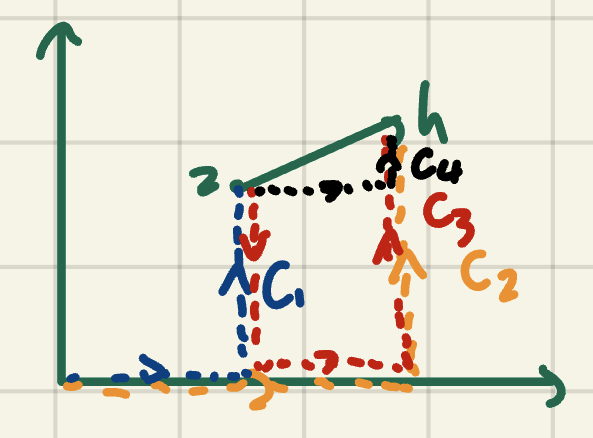
\includegraphics[width=0.2\textwidth]{img/integral_thm.png}
  \end{figure}

  \noindent Now, for $h \in \mathbb{C}$, we have $F(z + h) = \int_{C_1} f(z) dz$ and $F(z) = \int_{C_2} f(z) dz$. \\

  \noindent This means, \lghl{$F(z + h) - F(z) = \int_{C_1} f(\eta) d\eta + \int_{-C_2} f(\eta) d\eta = \int_{C_3} f(\eta) d\eta = \int_{C_4} f(\eta) d\eta$}. \\

  \noindent As \lghl{$\frac{1}{h} \int_{C_4} dz = 1$}, thus $(\frac{1}{h} \int_{C_4} f(\eta) d\eta) - f(z) =$ \lghl{$\frac{1}{h} \int_{C_4} (f(\eta) - f(z)) d\eta = \frac{F(z + h) - F(z)}{h} - f(z)$} \\

  \noindent In other words, by ML-formula, $\frac{F(z + h) - F(z)}{h} << \frac{1}{|h|} \varepsilon \cdot 2|h| \Rightarrow \lim_{h \to 0} \frac{F(z + h) - F(z)}{h} = f(z)$
\end{proof}

\pinkbox{Corollary}{
  If $f$ is entire and $C$ is a \textbf{smooth closed curve}, then \hl{$\int_C f(z) dz = 0$}
}

\pinkbox{Rectangle Theorem II}{
  Let $f$ be entire, and

  \[
    g(z) :=
    \begin{cases}
      {\textcolor{red}{\boxed{\dfrac{f(z) - f(a)}{z - a}}}}, & z \neq a, \\[6pt]
      f'(a), & z = a,
    \end{cases}
    \quad \text{which is continuous (since $f$ entire $\Rightarrow$ $g$ continuous).}
  \]

  Then, \hl{$\int_\Gamma g(z) dz = 0$}, where $\Gamma$ is a boundary of a closed rectangle $R \subseteq \mathbb{C}$
}

\begin{proof}
  As $g$ is conti, by def, $\exists M \in \mathbb{R}$, s.t. $|g(z)| < M\ \forall z \in \mathbb{R}$

  \begin{enumerate}
    \item \lghl{If $a \in \mathbb{C} \setminus R$}, then $g(z)$ is \textbf{analytic for all $\mathbf{z \in R}$}. Hence, by the argument of the Rectangle Thm, $\int_\Gamma g(z) dz = 0$
    \item \lghl{If $a \in \Gamma$}, where $\Gamma_i :=$ boundary of $R_i$
    \begin{figure}[h]
      \centering
      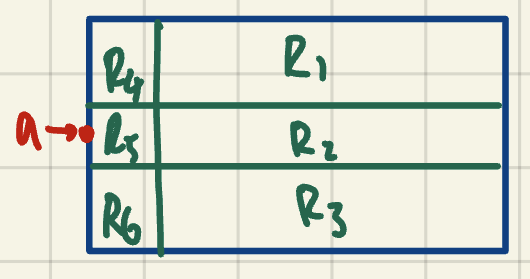
\includegraphics[width=0.20\textwidth]{img/case2_rect2.png}
    \end{figure}

    Then, by case 1, $\int_\Gamma g(z) dz =$ \lghl{$\int_{\Gamma_s} g(z) dz << M \cdot 4\varepsilon$} by the ML-formula, with $M$ indep of $\varepsilon$, where we define $\varepsilon$ to be the length of the \textbf{longest side} of $\Gamma_s$. Hence, as \lghl{$\varepsilon \to 0$, $\int_\Gamma g(z) dz = 0$}
    \item \lghl{Otherwise, $a \in$ interior of $R$}. Then we have:

    \vspace{0.4em}\begin{figure}[h]
      \centering
      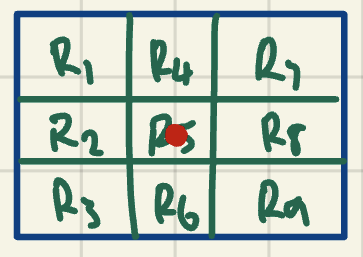
\includegraphics[width=0.15\textwidth]{img/case3_rect2.png}
    \end{figure}

    Then, by case 1, $\int_\Gamma g(z) dz=$ \lghl{$\int_{\Gamma_s} g(z) dz << M \cdot 4\varepsilon \to 0$} as $\varepsilon \to 0$
  \end{enumerate}
\end{proof}

\bluesec{Cauchy Integral Formula}

\pinkbox{Lemma}{
  Define $C_\rho(\alpha) :=$ circle centered at $\alpha$ with radius $\rho$, where $\alpha$ may be omitted if there is no amibiguity. Then, \hl{$I := \int_{C_\rho(\alpha)} \frac{dz}{z - a} = 2 \pi i$} $\forall |a - \alpha| < \rho$
}

\begin{proof}
  If $a = \alpha$, then it's clear, since $C_\rho(\alpha) = \alpha + \rho e^{i \theta}$, $0 \leq \theta 2\pi$. \\

  \noindent For $a \neq \alpha$, we know $\boxed{I = \int_{C_\rho(\alpha)} \frac{dz}{(z - \alpha) - (a - \alpha)} = \int_{C_\rho(\alpha)} \frac{1}{z - a} \cdot \frac{1}{1 - \frac{a - \alpha}{z - \alpha}} dz}$ \\

  \noindent Notice, $\forall z \in C_\rho(\alpha)$, $|\frac{a - \alpha}{z - \alpha}| < 1$. Hence, we have \lghl{unif conv: $(1 - \frac{a - \alpha}{z - \alpha})^{-1} = 1 + (\frac{a - \alpha}{z - \alpha}) + (\frac{a - \alpha}{z - \alpha})^2 + \dots$} \\

  \noindent Hence, $I = \int_{C_\rho{\alpha}} \frac{1}{z - \alpha}(\sum_{k = 0}^\infty (\frac{a - \alpha}{z - \alpha})^k) dz = \sum_{k = 0}^\infty \int_{C_\rho(\alpha)} \frac{1}{z - \alpha} (\frac{a - \alpha}{z - \alpha})^k dz$. \\

  \noindent We now consider \lghl{$J_k := \int_{C_\rho(\alpha)} \frac{1}{(z - \alpha)^k} dz$}. When $k = 1$, thus $J_1 = 2\pi i$. When $k > 1$, $J_k = \int_0^{2\pi} \frac{i e^{i \theta}}{\rho^k e^{i k \theta}} d\theta = \int_0^{2\pi} \frac{i}{\rho^k} e^{i\theta(k - 1)} d\theta = 0$. Hence, \lghl{$I = 2\pi i$}.
\end{proof}

\pinkbox{Cauchy Integral Formula}{
  Given an entire $f$, $a \in \mathbb{C}$, $C = Re^{i\theta},\ 0 \leq \theta \leq 2 \pi$ with $a$ within the unit disc of radius $R$, then we have \hl{$f(a) = \frac{1}{2\pi i}\int_C \frac{f(z)}{z - a} dz$}
}

\begin{proof}
  By rectangle thm 2, we know \lghl{$\int_C g(z) dz = \int_C \frac{f(z)}{z - a} - \frac{f(a)}{z - a} dz = 0$}. Thus, $\int_C \frac{f(z)}{z - a} dz = \int_C \frac{f(a)}{z - a} dz =$ \lghl{$f(a)\int_C \frac{1}{z - a} dz = f(a) 2\pi i$}
\end{proof}

\vspace{1.0em}\bluesec{Taylor Expansion}

\pinkbox{Taylor Expansion for Entire Function}{
  Given $f$ is an entire function, then $f^{(k)}(0)$ exists $\forall k \in \mathbb{Z}_{> 0}$ and \hl{$f(z) = \sum_{k = 0}^\infty \frac{f^{(k)}(0)}{k!} z^k$} $\forall z \in \mathbb{C}$
}

\begin{proof}
  \begin{figure}[h]
    \centering
    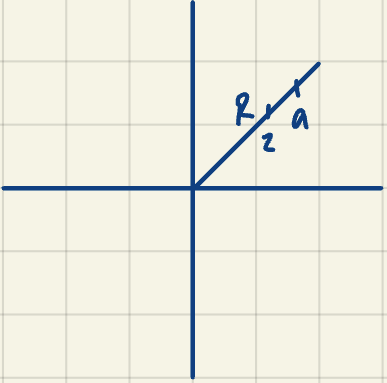
\includegraphics[width=0.2\textwidth]{img/taylor.png}
  \end{figure}

  \noindent Choose $a \in \mathbb{C}$, $|a| > |z|$, $\boxed{R := |a| + 1}$. By Cauchy Integral Formula, \lghl{$f(z) = \frac{1}{2\pi i} \int_{C_R} \frac{1}{1 - \frac{z}{w}} \frac{f(\omega)}{\omega} d\omega$}. \\

  \noindent As $|\frac{z}{\omega}| < \frac{|a|}{1 + |a|}$, then \lghl{$f(z) = \sum_{k = 0}^\infty \int_{C_R} \frac{f(\omega)}{\omega} (\frac{z}{\omega})^k d\omega = \sum_{k = 0}^\infty z^k \int_{C_R} \frac{f(\omega)}{\omega^{k + 1}} d\omega = \sum_{k = 0}^\infty z^k C_k$}. \\

  \noindent Notice, as $|z| < |a|$, then \lghl{$f'(z) = \sum_{i = 1}^\infty i z^{i - 1} C_i \Rightarrow f'(0) = C_1$}. If we continue this process, thus $f^{(k)}(0)$ exists $\forall k \in \mathbb{N}_{> 0}$ and $f(z) = \sum_{k = 0}^\infty \frac{f^{(k)}(0)}{k!} z^k$
\end{proof}

\pinkbox{Corollary}{
  Let $f$ be an entire function with zeros at $a_1, \dots, a_N$. Define \hl{$g(z) = \frac{f(z)}{(z - a_1) \cdots (z - a_N)}$} for $z \notin \{a_1, \dots, a_N\}$. Then, $\lim_{z \to a_i} g(z)$ exists $\forall i$. If we define \hl{$g(a_i) := \lim_{z \to a_i} g(z)$}, then $g$ is \textbf{entire}.
}

\begin{proof}
  Set $f_0 = f$, and \lghl{$f_k := \frac{f_{k - 1}(z) - f_{k - 1}(a_k)}{z - a_k}$}. Hence, $f_1$ is entire. By recurrence, $g$ is entire.
\end{proof}

\vspace{1.0em}\bluesec{Liouville's Theorem}

\pinkbox{Liouville's Theorem}{
  \textbf{Entire bounded} functions on $\mathbb{C}$ are \textbf{constants}.
}

\begin{proof}
  Let $a \in \mathbb{C} \setminus \{0\}$ and consider $R > |a|$. \\

  \noindent Then, by Cauchy Integral Formula, \lghl{$f(a) - f(0) = \frac{1}{2\pi i} \int_{C_R} \frac{f(z)}{z - a} - \frac{f(z)}{z} dz = \frac{1}{2 \pi i} \int_{C_R} \frac{af(z)}{z (z - a)} dz$}. \\

  \noindent As $f$ is \textbf{bounded}, $\exists M \in \mathbb{R}_{> 0}$, s.t. \lghl{$|f(z)| < M$} $\forall z \in \mathbb{C}$. \\

  \noindent By ML-formula, \lghl{$|f(a) - f(0)| < \frac{1}{2 \pi i} (\frac{M \cdot |a|}{R(R - |a|)} \cdot 2\pi R) \to 0$} as $R \to \infty$. Hence, $\boxed{f(a) = f(0)}\ \forall a \in \mathbb{C}$.
\end{proof}

\pinkbox{Extended Liouville's Theorem}{
  Given $f$ is entire. Suppose \hl{$|f(z)| < A + B|z|^k$} for some constants $A, B \in \mathbb{R}_0$. Then, $f$ is a polynomial with \textbf{degree at most k}
}

\begin{proof}
  We consider induction on $k$. By Louville's Thm, we already know $k = 0$ is true. \\

  \noindent For \lghl{$k > 0$}, define the \textbf{entire} function
  \[
    g(z) :=
    \begin{cases}
      {\textcolor{red}{\boxed{\dfrac{f(z) - f(0)}{z}}}}, & z \neq 0, \\[6pt]
      f'(0), & z = 0,
    \end{cases}
  \]

  \noindent As $|f(z)| < A + B|z|^k$ is \textbf{bounded}, define \lghl{$M_0 := \max_{z \in C_R}g(z)$} for some $R \geq 1$. Thus, we have for \lghl{$z \in \mathbb{C} \setminus C_R, |g(z)| < A + B|z|^{k - 1}$} and for \lghl{$z \in C_R,\ |g(z)| < M_0$}. This means, $\exists\ D, E \in \mathbb{R}_{>0}$, s.t. \\ $\boxed{|g(z)| < D + E|z|^{k - 1}}$ \\

  \noindent Hence, $g$ is a poly of degree \textbf{at most k -- 1}, i.e. $f$ is a poly of degree \textbf{at most k}.
\end{proof}

\pinkbox{Fundamental Theorem of Algebra}{
  Nonconstant polynomials have roots in $\mathbb{C}$
}

\begin{proof}
  Consider a polynomial $p(x)$. Suppose $p$ has \textbf{no roots} in $\mathbb{C}$. \\

  \noindent Then, \lghl{$f(z) := \frac{1}{p(z)}$} is \textbf{entire}. Moreover, as $z \to \infty$, $|f(z)| \to 0$, so $|f(z)|$ is \textbf{bounded}. \\

  \noindent Hence, by Louville's Thm, $f(z)$ is const $\Rightarrow p(z)$ is constant, which is a contradiction.
\end{proof}

\pinkbox{Gauss-Lucas Theorem}{
  The \textbf{zeros of the derivative of a polynomial} lie within the \textbf{convex hull} of the \textbf{zeros} of the polynomial.
}

\begin{proof}
  Let $p(x)$ be a nonconstant polynomial in $\mathbb{C}[x]$, and $\alpha_1, \dots, \alpha_n$ be the \textbf{roots} of $p$ counted by multiplicity. Then, \lghl{$p(x) = c \Pi_{i = 1}^n (x - \alpha_i)$}. Moreover, \lghl{$\frac{p'(x)}{p(x)} = \sum_{i = 1}^n \frac{1}{x - \alpha_i}$}. \\

  \noindent Let $a$ be a root of $p'(x)$ and $a \notin \{\alpha_1, \dots \alpha_n\}$. Then, $\frac{p'(a)}{p(a)} = \sum_{i = 1}^n \frac{1}{a - \alpha_i} = \sum_{i = 1}^n \frac{\bar{a} - \bar{\alpha_i}}{|a - \alpha_i|^2}$, so $\bar{a} = \sum_{i = 1}^n c_i \bar{\alpha_i}$, where \lghl{$c_i = \frac{1}{|a - \alpha_i|^2} / \sum_{i} \frac{1}{|a - \alpha_i|^2} \in \mathbb{R}_{\geq 0}$}. \\

  \noindent Hence, $a = \sum_{i = 1}^n c_i \alpha_i$, $c_i \in \mathbb{R}_{\geq 0}, \sum c_i = 1$, so by def, this concludes the proof.
\end{proof}

\vspace{1.0em}\bluesec{Uniqueness, Mean Modulus, Max/Min Modulus Theorems}

\purplesec{Uniqueness Theorem}

\noindent Remark: We can only apply the following theorems below, including max/min modulus thm, only when its \textbf{acc points are in D}. \\

\pinkbox{Uniqueness Theorem}{
  Say $D$ is a \textbf{region} and $f$ is an \textbf{analytic region} on $D$. Suppose that $\exists$ seq of distinct \hlbf{zeros} of $D$ $\{z_n\}$, s.t. \hl{$\lim_{n \to \infty} z_n = z_0 \in D$}, where we say the seq $\{z_n\}$ has an \textbf{acc pt} in $D$. Then, \hl{$f \equiv 0$} on $D$.
}

\begin{proof}
  As we know, $f$ is ana, so it is conti, i.e. \lghl{$f(z_0) = \lim_{n \to \infty} f(z_n) = 0$}. \\

  \noindent Define $A := \{z \in D\ |\ z \text{ is an \textbf{acc point of zeros} of $f$ in $D$}\}$

  \begin{itemize}
    \item \lghl{``$A$ is open''}: By uniqueness of power series, $f \equiv 0$ in some disk $D(z, \delta_z) \subseteq D\ \forall z \in A$, i.e. $D(z, \delta_z) \subseteq A\ \forall z \in A$.
    \item \lghl{``$D \setminus A$ is open''}: $z$ is \textbf{NOT an acc point of zeros} $\Rightarrow \exists$ open nbd $U$ of $z$ in $D$ s.t. $f(z)$ has \textbf{NO zeros} in $U \setminus \{z\}$. As $f$ is conti, $\forall y \in U \setminus \{z\}, \exists$ open nbd $V_y \subseteq D$ of $y'$, s.t. \lghl{$f \neq 0$ on $V_y \Rightarrow y \in D \setminus A$}
  \end{itemize}

  \noindent Hence, $z_0 \in A$ and $D$ is a region, with $D = A$
\end{proof}

\pinkbox{Polynomials}{
  If $f$ is \textbf{entire} and \hl{$f \to \infty$ as $z \to \infty$}, then $f$ is a \hlbf{polynomial}.
}

\begin{proof}
  By def, $\forall M \in \mathbb{R}_{> 0}, \exists \delta$, s.t. $\forall |z| > \delta$, \lghl{$|f(z)| > M$}. \\

  \noindent Let $M = 1$. Thus, $\exists\ \delta$, s.t. $\forall |z| > \delta, |f(z)| > 1$. By assumption, $f$ is \textbf{NOT constant}. \\

  \noindent \textbf{Claim:} \lghl{$f$ has \textbf{finitely many zeros}}
  \begin{proof}
    By $\delta$, all zeros in $f$ are in $\overline{D(0, \delta)}$, otherwise, $|f(z)| \neq 0$. As $\overline{D(0, \delta)}$ is cpt, \lghl{$\exists$ acc pt of zeros in} \lghl{$\overline{D}(0, \delta) \Rightarrow f \equiv 0$ on $D(0, \delta')$} for all $\delta' > \delta$, which is a contradiction.
  \end{proof}

  \noindent Now consider within $\bar{D}(0, \delta)$. Let $\alpha_1, \dots, \alpha_N$ be the zeros of $f$. Then, \lghl{$g(z) = f(z) / \Pi_{i = 1}^n (z - \alpha_i)$ is \textbf{entire}} \lghl{and has \textbf{no zeros} in $\mathbb{C}$}. \\

  \noindent Set \lghl{$h(z) := \frac{1}{g(z)}$}, then $h$ is \textbf{entire} and is \textbf{bounded} in the disk. \\

  \noindent By Extended Liouville's Thm, thus \lghl{$|h| < A + B|z|^n$} for all $|z| > \delta$ (By $|f(z)| > 1 \Rightarrow |h(z)| < \Pi_{i = 1}^n (z - \alpha i)$) and $|z| \leq \delta \Rightarrow h$ is a poly. \\

  \noindent However, \lghl{$h$ has \textbf{no zeros}} in $\mathbb{C}$. Thus, $h$ is \textbf{const}. \\

  \noindent $\therefore \exists\ c \in \mathbb{C}^\times$, s.t. \lghl{$f(z) = c  \Pi_{i = 1}^n (z - \alpha_i)$}
\end{proof}

\vspace{1.0em}\purplesec{Mean Modulus Theorem}

\pinkbox{Mean Value Theorem}{
  Let $D$ be a region, $f$ ana on $D$, $\alpha \in D$. Then, \hl{$f(\alpha)$ = mean value of $f$} taken around the \textbf{boundary} of \textbf{any disk centered at $\mathbf{\alpha}$ and contained at $\mathbf{D}$}
}

\begin{proof}
  By Cauchy-Integral Formula, \lghl{$f(\alpha) = \frac{1}{2\pi i} \int_{C_\delta(\alpha)} \frac{f(z)}{z - \alpha} dz$}. Say \lghl{$z = \alpha + \delta e^{i \theta}$ for $\theta \in [0, 2\pi]$}, we get \lghl{$f(\alpha) = \frac{1}{2\pi} \int_0^{2\pi} f(\alpha + \delta e^{i\theta}) d\theta$}
\end{proof}

\vspace{1.0em}\purplesec{Max/Min Modulus Theorem}

\pinkbox{Maximum Modulus Theorem}{
  Say $f$ is \textbf{nonconst}, ana on a region $D$. Then, $\forall z \in D$ and $\delta \in \mathbb{R}_{\geq 0}$, $\exists$ some $\omega \in D(z, \delta) \cap D$, s.t. $|f(\omega)| > |f(z)|$
}

\begin{proof}
  By MVT, \lghl{$f(z) = \frac{1}{2\pi} \int_0^{2\pi} f(z + \delta e^{i\theta}) d\theta$} for small enough $\delta$ s.t. $D(z, \delta) \subseteq D$. \\

  \noindent Then, by ML-formula \lghl{$|f(z)| {\textcolor{red}{\leq}} \frac{1}{2\pi} \max_{\theta \in [0, 2\pi]} |f(z + \delta e^{i \theta})| \cdot 2\pi = \max|f(z + \delta e^{i\theta})|$} \\

  \noindent When ${\textcolor{red}{\leq}}$ has equality, then $|f(z + \delta e^{i\theta})| = \max |f(z + \delta e^{i \theta})| \Rightarrow f$ is \textbf{const} on $C_\delta(z) \subseteq D$. As $f$ agrees with $g \equiv \text{const}$ \textbf{on a set of points with acc point}, $f$ is const on $D$. \\

  \noindent However, $f$ is nonconst. Hence, \lghl{$|f(z)| {\textcolor{red}{<}} \max_{\theta \in [0, 2\pi]} |f(z + \delta e^{i \theta})|$}
\end{proof}

\pinkbox{Minimum Modulus Theorem}{
  Say $f$ is nonconst and ana on a region D, $\forall\ z \in D, f(z) \neq 0$. Then, $f$ has \textbf{no interior min points}.
}

\begin{proof}
  Let \lghl{$g(z) := \frac{1}{f(z)}$}. Observe, $g$ is ana and nonconst on $D$. By max modulus thm, we proved it.
\end{proof}

\vspace{1.0em}\bluesec{Saddle Points}

\pinkbox{Theorem on Maxima}{
  Say $\bar{D}$ is a \textbf{closed disk (circle)} and $f$ is analytic and nonconst on $\bar{D}$. $f$ assumes its \textbf{max value} at a boundary point $z_0$, then \hl{$f'(z_0) \neq 0$}
}

\begin{proof}
  Suppose $f'(z_0) = 0$. \\
  
  \noindent Then, $f(z_0 + \delta) \approx f(z_0) + \frac{1}{2} f''(z_0) \xi^2$ \lghl{$\Rightarrow|f(z_0 + \delta)|^2 = |f(z_0)|^2 + \frac{2}{k!}\Re(\bar{f}(z_0) f^{(k)}(z_0) x^k) + \dots$} for some $k \geq 2$. \\

  \noindent Let \lghl{$e^{i \theta} = \frac{\xi}{|\xi|}$}. Then, $\bar{f}(z_0) f^{(k)}(z_0) = Ae^{i\alpha} \Rightarrow$ \lghl{$|f(z_0 + \xi)|^2 - |f(z_0)|^2 = \frac{2}{k!}A|\xi|^k \cos(\alpha + k\theta) + \dots$}. \\

  \noindent As $|f(z_0)|$ is \textbf{max}, hence \lghl{$|f(z_0 + \xi)|^2 - |f(z_0)|^2 \leq 0\ \forall z_0 + \xi \in D$}, in other words, for small enough $\xi$, \\ 
  
  \noindent\lghl{$\cos(k\theta + \alpha) \leq 0 \Rightarrow \frac{\frac{\pi}{2} - \alpha}{k} + \frac{2\pi j}{k} \leq \theta \leq \frac{\frac{3}{2}\pi - \alpha}{k} + \frac{2\pi j}{k}$} for $0 \leq j \leq k - 1$. \\

  \noindent However, for a disc, $\exists\ \xi$, s.t. $z_0 + \xi$ is NOT in any one of the cones, since $\frac{\pi}{k} \leq \frac{\pi}{2}$. Thus, there is a contradiction.
\end{proof}

\pinkbox{Theorem on Saddle Points}{
  $z_0$ is a \textbf{saddle point} of an analytic function $f$ iff \hl{$f'(z_0) = 0$ and $f(z_0) \neq 0$}
}

\begin{proof}
  We have $z = x + iy, f(z) = u(x, y) + iv(x, y)$, and $g(z) = \sqrt{u^2 + v^2} \geq 0$

  \begin{itemize}
    \item ``$\Rightarrow$'': As $g(z_0)$ is not a local minimum, hence \lghl{$g(z_0) \neq 0$, so $u(z_0) \neq 0$ or $v(z_0) \neq 0$} \\
    
    We know \lghl{$g_x(z_0) = g_y(z_0) = 0$} $\Rightarrow \frac{uu_x + vv_x}{g}|_{z_0} = \frac{uu_y + vv_y}{g}|_{z_0} = 0$, i.e. \lghl{$\begin{bmatrix}
      u_x(z_0) & v_x(z_0) \\
      u_y(z_0) & v_y(z_0)
    \end{bmatrix} \begin{bmatrix}
      u(z_0) \\
      v(z_0)
    \end{bmatrix}$ = 0} \\

    However, by CR-eq, $\det\begin{bmatrix}
      u_x(z_0) & v_x(z_0) \\
      u_y(z_0) & v_y(z_0)
    \end{bmatrix} = u_x^2(z_0) + v_x^2(z_0)$. Hence, \lghl{$u_x(z_0) = v_x(z_0) = 0$} \\

    As $f$ is ana, hence $f'(z_0) = 0$. From above with $g(z_0) \neq 0$, we also know $f(z_0) \neq 0$.

    \item ``$\Leftarrow$'': As $f'(z_0) = 0$, thus $u_x(z_0) = v_x(z_0) = u_y(z_0) = v_y(z_0) = 0$, i.e. \lghl{$g_x(z_0) = g_y(z_0) = 0$}. However, by the \textbf{max and min modulus thms}, \lghl{$|f(z_0)|$ is NOT a local extremum}.
  \end{itemize}
\end{proof}

\bluesec{Oppen Mapping Theorem and Schwarz Lemma}

\purplesec{Open Mapping Theorem}

\pinkbox{Open Mapping Theorem}{
  $\forall$ \hl{\textbf{open set} $\mathbf{U \subseteq D}$, $\mathbf{f(U)}$ is also \textbf{open}} in $\mathbb{C}$ for any nonconst \textbf{ana} $f$.
}

\begin{proof}
  It suffices to show \lghl{$\forall \beta = f(\alpha') \in f(D(\alpha, \varepsilon)), \exists D(\beta, \varepsilon') \subseteq f(D(\alpha, \beta))$}. \\

  \noindent WLOG, we can assume \lghl{$f(\alpha) = 0$}, so we choose $\varepsilon$ s.t. \lghl{$\overline{D(\alpha, \varepsilon)} \subseteq D$}. By uniqueness thm, $\exists s$, s.t. $f$ has \lghl{\textbf{no zeros} in $\overline{D(\alpha, \varepsilon)} \setminus \{\alpha\}$ or else $f \equiv 0$}. \\

  \noindent Let $2\delta = \min_{z \in C_\varepsilon(\alpha)} |f(z)| > 0$ \\

  \noindent \textbf{Claim:} $D(f(\alpha) = 0, \delta) \subseteq Im(f)$

  \begin{proof}
    $\forall w \in D(0, \delta)$, consider $f(z) - w$. \\

    \noindent If $w \notin f(D(\alpha, \varepsilon))$, then \lghl{$f(z) - w$ \textbf{has no zeros}} on $D(\alpha, \varepsilon)$. \\

    \noindent Hence, \lghl{$|f(z) - w| \geq |f(z)| - |w| \geq \delta$} $\forall z \in C_\varepsilon(\alpha)$. However, we know \lghl{$|f(\alpha) - w| < \delta$}, which is a contradiction.
  \end{proof}

  \noindent Thus, $w \in f(D(\alpha, \varepsilon)) \Rightarrow D(0, \delta) \subseteq Im(f)$
\end{proof}

\newpage

\purplesec{Schwarz Lemma}

\pinkbox{Schwarz Lemma}{
  Suppose that $f$ is analytic in an \textbf{open unit disc} $D$ with \hl{$|f| \leq 1$ and $f(0) = 0$}. Then,

  \begin{enumerate}
    \item \hl{$|f(z)| \leq |z|$}
    \item \hl{$|f'(0)| \leq 1$}
  \end{enumerate}

  with equality in either of the above iff \hl{$f(z) = e^{i\theta} z$}
}

\begin{proof}
  Define $g(z) = \begin{cases}
    {\textcolor{red}{\frac{f(z)}{z}}}, \quad &z \neq 0 \\
    f'(z), &z = 0
  \end{cases}$

  \noindent $g(z)$ is ana on $D$ since $f(z)$ is ana on D. \\

  \noindent Consider \lghl{$z \in C_r(0)$} for $0 < r < 1$, then \lghl{$|g(z)| = \frac{|f(z)|}{|z|} \leq \frac{1}{r}$} \\

  \noindent By \textbf{max modulus thm}, $\forall z \in \overline{D(0, r)}, |g(z)| \leq \frac{1}{r}$. As $r \to 1$, then \lghl{$|g(z)| \leq 1\ \forall z \in D$}. \\

  \noindent \lghl{By def of $g(z)$}, $|f(z)| \leq |z|$ and $|f'(0)| \leq 1$ has either equality hold, when \lghl{$g$ is const and $|g| = 1$} on $D$. Hence, $g = e^{i\theta}$.
\end{proof}

% Rmb to do the B_alpha thing in definitions idk

\pinkbox{Proposition}{
  Say $f$ is \textbf{entire}. If \hl{$|f(z)| < \frac{1}{|\Im(z)|}$} for all $z$, then \hl{$f \equiv 0$}
}

\begin{proof}
  Define \lghl{$g(z) = (z^2 - R^2)f(z)$}, for some $R \in \mathbb{R}_{> 0}$ (sufficiently large, e.g. $R \geq 1, R \to \infty$). \\

  \noindent When $z \in C_R(0)$, \lghl{$|z - R||z + R| \leq 2R |\Im(z)|$}. Hence, \lghl{$|g(z)| \leq \frac{2R}{|\Im(z)|^2} \leq 2R$} when $z \in C_R(0)$ \\

  \noindent By max modulus thm, \lghl{$|g(z)| \leq 2R\ \forall z \in D(0, R)$}. Hence, $\forall z \in D(0, R), |f(z)| \leq \frac{2R}{|z^2 - R^2|} \to 0$ as $R \to \infty$. Thus, \lghl{$f(z) = 0$}
\end{proof}

\vspace{1.0em}\bluesec{Morera's Theorem}

\purplesec{Morera's Theorem}

\pinkbox{Morera's Theorem}{
  Let $f$ be \textbf{continuous} on an open set $D \subseteq \mathbb{C}$ and $\Gamma$ be the boundary of a \textbf{closed rectangle} $R \subseteq D$. If \hl{$\int_\Gamma f dz = 0\ \forall\ \Gamma \in R \subseteq D$, then $f$ is \textbf{analytic} in $D$}.
}

\begin{proof}
  Say $z_0 \in D$, where $D$ is open. Then, $\exists \varepsilon > 0$, s.t. \lghl{$D(z_0, \varepsilon) \subseteq D$}. \\

  \noindent Define \lghl{$F(z) := \int_C f(z) dz$} $\forall z \in D(z_0, \varepsilon)$, where $C: z_0 \to z_0 + \Re(z - z_0) \to z$. \\

  \noindent For $z \in D(z_0, \varepsilon)$ and $k$ \lghl{small enough s.t. $z + h \in D(z_0, \varepsilon)$}, then: \\
  
  \noindent \lghl{$\lim_{h \to 0} \frac{F(z + h) - F(z)}{h} = \lim_{h \to 0} \int_{C_1} f(\omega) d\omega = f(z)$}

  % \begin{figure}[h]
  %   \centering
  %   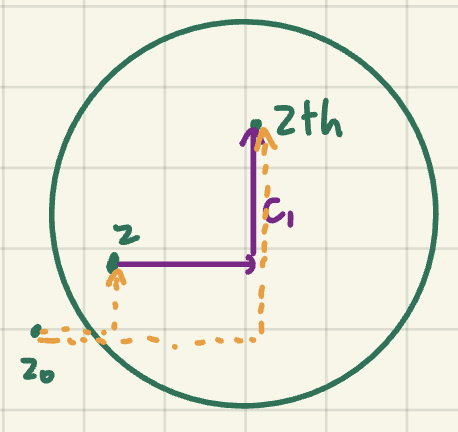
\includegraphics[width=0.2\textwidth]{img/morera.png}
  % \end{figure}
\end{proof}

\pinkbox{Corollary}{
  Let $D$ be an open set in $\mathbb{C}$ and $\{f_n\}$ be a sequence of ana functions s.t. \hl{$f_n \to f$ unif on cpta}. Then, $f$ is also \textbf{ana in D}.
}

\begin{proof}
  As $f_n$ is conti $\forall K \subseteq D$ that is a cpt set, we have $f_n \to f$ unif on K. Thus, $f$ is conti on $K$ for all $K$, i.e. \lghl{$f$ is conti on $D$}. \\

  \noindent Notice, \lghl{$\int_\Gamma f dz = \int_\Gamma \lim_{n \to \infty} f_n dz = \lim_{n \to \infty}(\int_\Gamma f_n dz) = 0$}. Thus, by Morera's Thm, $f$ is conti.
\end{proof}

\purplesec{Schwarz Reflection Principle}

\pinkbox{Analytic Except on a Line Segment}{
  $f$ is continuous on an open set $D \subseteq \mathbb{C}$ and \textbf{analytic except on a line segment} in $D$. Then, $f$ is \textbf{analytic throughout D}.
}

\begin{proof}

  \begin{figure}[h]
    \centering
    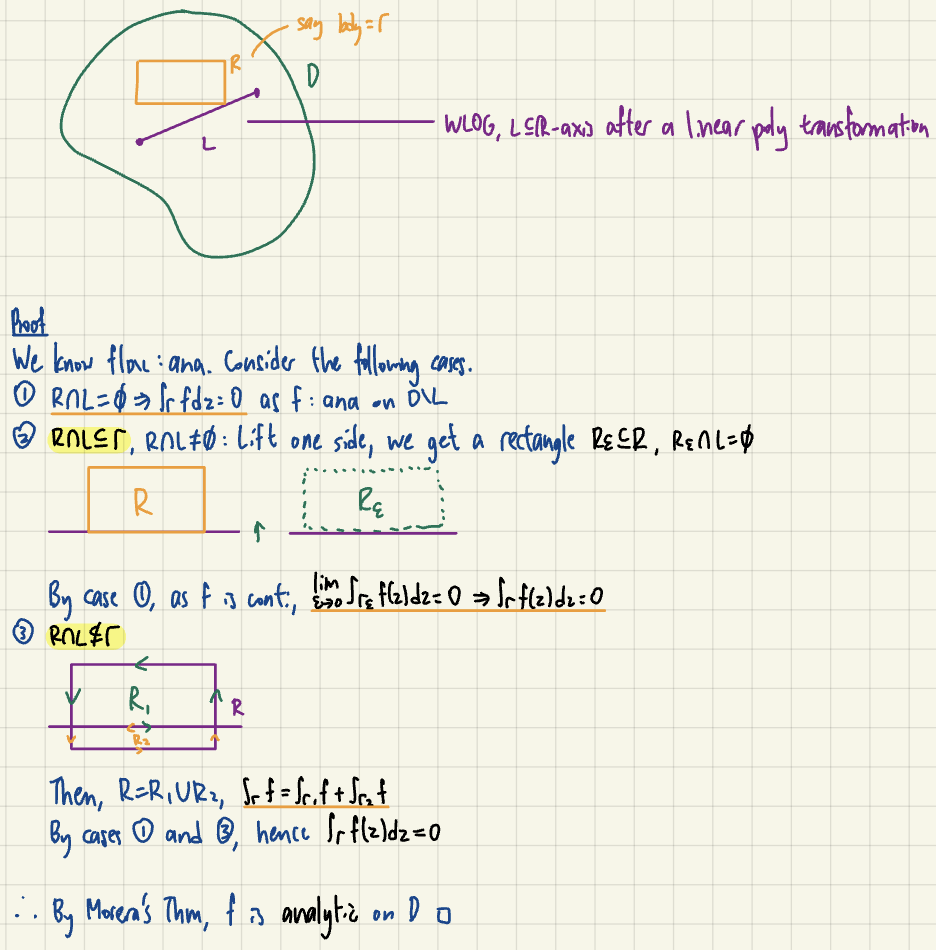
\includegraphics[width=0.65\textwidth]{img/except_for_line.png}
  \end{figure}

  \noindent (Note the image has a small typo, it should be ``by cases (1) and (2)'', not ``by cases (1) and (3)'', but I find it way easier to use that photo than to retype a mainly visual proof.)
\end{proof}

\pinkbox{Schwarz Reflection Principle}{
  Suppose $f$ is C-analytic on a region $D$ that is contained in either the upper or lower half plane and whose boundary contains a segment $L$ on the real axis, and suppose \hl{$f$ is real for real $z$}. \\

  Then, we can define an analytic ``extension'' $g$ of $f$ to the region $D \cup L \cup D*$ that is \textbf{symmetric} w.r.t. the real axis by:

  \hl{$g(z) = \begin{cases}
    f(z), &z \in D \cup L \\
    \overline{f(\overline{z})}, &z \in D*
  \end{cases}$,\quad where $D* = \{z\ |\ \bar{z} \in D\}$}
}

\begin{proof}
  We consider the proof for two main cases:

  \begin{enumerate}
    \item For any \lghl{$z \in D$}, then \lghl{$f|_D = g|_D$}, so $f$ ana implies $g$ is ana
    \item For any \lghl{$z \in D*$ and $z + h \in D*$}, we have 
    
    \noindent \lghl{$\lim_{h \to 0} \frac{g(z + h) - g(z)}{h} = \lim_{h \to 0} \overline{(\frac{f(\overline{z + h}) - f(\overline{z})}{\overline{h}})} = \overline{f'(\overline{z})}$, so $g$ is ana}
  \end{enumerate}

  \noindent As $f$ is conti on the $\mathbb{R}$-axis, so is $g$, so we can apply the theorem of ``analytic except for a line segment'', to determine \lghl{$g$ is ana throughout $D \cup L \cup D* = U$}
\end{proof}

\vspace{1.0em}\bluesec{Simply Connected Domain}

\noindent Although there are other theorems, I won't spend time proving them here because they all derive from this key lemma anyway. \\

\pinkbox{Key Lemma for Polygonal Curves}{
  Let $\Gamma$ be a simple closed polygonal curve bounding $D$ (simply connected). \\
  
  Then any \textbf{horizontal segment} joining two consecutive ``top-level'' intersection points of $\Gamma$ \hl{lies entirely inside $D$}.
}

\begin{proof}
  Here is a very rough proof that won't get you marks, I just don't have the time to summarize this proof, and I don't think it's tested (?).

  \noindent Induct on the \textbf{level} of $\Gamma$: \\
  
  \noindent Base: $\Gamma$ a rectangle, trivial. \\
  
  \noindent Inductive step: split $\Gamma$ into lower-level subcurves, show that the \lghl{horizontal strip between consecutive top} \lghl{levels stays inside $D$} (using path-connectedness and openness arguments).
\end{proof}

\vspace{1.0em}\bluesec{Analytic Branch}

\pinkbox{Analytic Branch for $\log$}{
  Set \hl{$f(z) := \int_{z_0}^z \frac{1}{\xi} d\xi + \log z_0$} on a s.c. region $D \subseteq \mathbb{C} \setminus \{0\}$, we fix a $z_0 \in D$ and choose $\log z_0$. Then, $f$ is an \textbf{analytic branch} of $\log z$ in $D$.
}

\begin{proof}
  As $D$ is s.c., choose a closed curve $C_1 - C_2$ (i.e. choose the endpoints and have two different paths). \\

  \noindent By closed curve thm, \lghl{$\int_{C_1 - C_2} \frac{1}{\xi} d\xi = 0 \Rightarrow \int_{C_1} \frac{1}{\xi} d\xi = \int_{C_2} \frac{1}{\xi} d\xi$}, thus $f$ is \textbf{analytic}. \\

  \noindent Moreover, we want ``$e^{f(z)} = z$'' $\Leftrightarrow$ ``$ze^{-f(z)} = 1$''. TL;DR, set $g(z) := ze^{-f(z)}$, then we get $g'(z) = 0$, so $g \equiv 1$.
\end{proof}

\vspace{1.0em}\bluesec{Singularity}

\pinkbox{Riemann's Principle of Removable Singularities}{
  (I don't want to waste time here, so let's just say it's the same as the poles of order $k$ thing below, except $k = 0$.)
}

\pinkbox{Poles of Order $k$}{
  Say $f$ has an \textbf{isolated singularity} at $z_0$. If $\exists k \in \mathbb{Z}_{>0}$, s.t. \hl{$\lim_{z \to z_0} (z - z_0)^k f(z) \neq 0$ but} \hl{$\lim_{z \to z_0} (z - z_0)^{k + 1} f(z) = 0$}, then $f$ has a \hl{pole of order $k$} at $z_0$.
}

\begin{proof}
  Set $g(z) = \begin{cases}
    {\textcolor{red}{\boxed{(z - z_0)^{k + 1} f(z)}}}, &z \in D'(z_0, \delta) = D(z_0, \delta) \setminus \{z_0\} \\
    0, &z = z_0
  \end{cases}$

  \noindent As $\lim_{z \to z_0} (z - z_0)^{k + 1} = 0$, thus $g$ is \lghl{conti at $\mathbf{z_0}$}. \\

  \noindent As $f$ is ana on $D'(z_0, \delta)$, $g$ is also \lghl{ana on $D'(z_0, \delta)$}. \\

  \noindent Hence, using the ``analytic except for a line'' theorem, we get \lghl{$g$ is ana on $D(z_0, \delta)$} \\

  \noindent Thus, set $h(z) := \begin{cases}
    {\textcolor{red}{\boxed{\frac{g(z) - g(z_0)}{z - z_0} = (z - z_0)^k f(z)}}}, &z \in D'(z_0, \delta) \\
    g'(z), &z = z_0
  \end{cases}$, \quad hence $h$ is ana on $D(z_0, \delta)$. \\

  \noindent As we know, \lghl{$\lim_{z \to z_0} h(z) = h(z_0) \neq 0$}. Thus, $f(z) = \frac{h(z)}{(z - z_0)^k}$ has a \lghl{pole of order $k$} at $z_0$.
\end{proof}

\pinkbox{Casorati-Weierstrass Theorem}{
  If $f$ has an \textbf{essential singularity} at $z_0$ and $D$ is a \textbf{deleted neighborhood} of $z_0$, whre $f$ is \textbf{analytic}, then the range \hl{$R := \{f(z)\ |\ z \in D\}$ is \textbf{dense}} in $\mathbb{C}$.
}

\begin{proof}
  Suppose not, then \lghl{$\exists \omega \in \mathbb{C}$ and $\delta > 0$, s.t. \textbf{open} $D(\omega, \delta) \cap R = \emptyset$}. \\

  \noindent I.e., $\forall z \in D, |f(z) - \omega| \geq \delta \Rightarrow |\frac{1}{f(z) - \omega}| \leq \frac{1}{\delta} \forall\ z \in D$. Thus, \lghl{$\frac{1}{f(z) - \omega}$ has a \textbf{removable singularity} at $z_0$}. \\

  \noindent Hence, $\exists$ ana $g$ on $D' \cup \{z_0\}$, s.t. $g(z) = \frac{1}{f(z) - \omega} \Rightarrow$ \lghl{$f(z) = \omega + \frac{1}{g(z)}$} $\forall\ z \in D'$. \\

  \noindent Hence, $z_0$ is a zero of $g(z)$ of \lghl{finite order $n$} or \lghl{$g(z_0) \neq 0$}. Thus, $f(z)$ has a \lghl{pole of order $\geq n$} at $z_0$, so it is not an \textbf{essential singularity}.
\end{proof}

\end{document}